% !TEX root = handbook-physics.tex
%!TEX TS-program = pdflatex
%!TEX encoding = UTF-8 Unicode


\chapter{Dynamics of Rotary Motion}
\label{ch-04}
\zhtitle{转动动力学}

\section{Moment of Force and Angular Momentum}
\label{sec-4.1}
\zhtitle{力矩与角动量}
\subsection{}\label{4.1.1} The moment of force, or force moment is a concept introduced in mechanics to characterize the external mechanical action exerted on a body that changes its rotary motion. Dis­tinction is made between the moment of force about a fixed point and about a fixed axis.
\zhpar{力矩是力学中引入的一个概念，用以表征改变物体转动运动的外部机械作用。力矩可分为对定点的力矩和对定轴的力矩两种情形加以区分。}

The \redem{moment of the force $\vb{F}$ about a fixed point $O$} (the \redem{pole}) is the vector quantity $\vb{M}$, equal to the vector product of the radius vector $\vb{r}$, from point $O$ to point $A$ of force application (\figr{fig-04-01}), by
the force vector $\vb{F}$: 
\zhpar{\redem{力 $\vb{F}$ 对定点 $O$ 的力矩}（称 $O$ 为\redem{极点}）是一个矢量 $\vb{M}$，它等于从点 $O$ 指向力的作用点 $A$ 的位矢 $\vb{r}$（见\figr{fig-04-01}）与力矢量 $\vb{F}$ 的矢积，如下式所示。}
\begin{equation*}%
\vb{M} = \qty[\vb{r\,F}].
\end{equation*}
\begin{marginfigure}%[!ht]
%\begin{wrapfigure}{r}{0.5\linewidth}
\centering
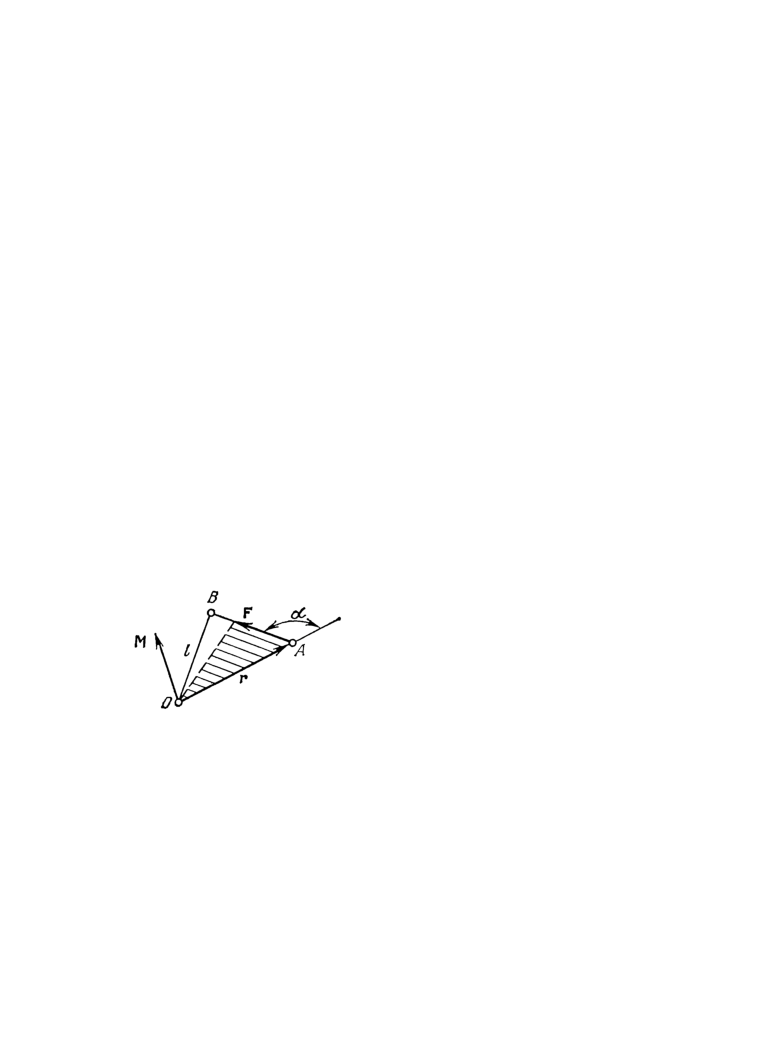
\includegraphics[width=0.8\textwidth,angle=-1]{figs/ch-04/fig-04-01.pdf}
%\input{figs/ch-03/fig-03-01}
%  \vspace{-13pt}
\sidecaption{The moment of force $\vb{M}$.\zhcap{力矩 $\vb{M}$ 的示意图。}
\label{fig-04-01}}
\end{marginfigure}
The magnitude of the moment of force is $M = Fr \sin \alpha = F l$, where $\alpha$ is the angle between vectors $\vb{r}$ and $F$, and $l = r \sin \alpha$ is the length of the perpendic­ular $OB$ (\figr{fig-04-01}) dropped from point $O$ to the line of action of the force. The quantity $l$ is called the \redem{arm of the force} with respect to point $O$. If the point of application of force $\vb{F}$ is displaced along its line of action, the moment $\vb{M}$ of this force about the same fixed point $O$ is not changed. If the line of action of the force passes through point $O$, the moment of the force about point $O$ equals zero.
\zhpar{力矩的大小为 $M = Fr \sin \alpha = F l$，式中 $\alpha$ 为矢量 $\vb{r}$ 与 $F$ 之间的夹角，$l = r \sin \alpha$ 为由点 $O$ 向力的作用线所作垂线 $OB$（见\figr{fig-04-01}）的长度。量 $l$ 称为力对点 $O$ 的\redem{力臂}。若力 $\vb{F}$ 的作用点沿其作用线移动，则该力对同一定点 $O$ 的力矩 $\vb{M}$ 保持不变。若力的作用线通过点 $O$，则该力对点 $O$ 的力矩等于零。}

\subsection{}\label{4.1.2} The \redem{principal}, or \redem{resultant, moment} of a system of forces \redem{about fixed point} $O$ (\redem{pole}) is the vector $\vb{M}$, equal to the geometric sum of the moments about point $O$ of all $n$ forces of the system:
\zhpar{力系\redem{对定点 $O$}（\redem{极点}）的\redem{主力矩}，或称\redem{合力矩}，是一个矢量 $\vb{M}$，它等于该力系中全部 $n$ 个力对点 $O$ 的力矩的几何和，如下式所示。}
\begin{equation*}%
\vb{M} = \sum_{i=1}^{n} \qty[\vb{r}_{i}\vb{F}_{i}],
\end{equation*}
where $\vb{r}_{i}$ is the radius vector from point $O$ to the point of appli­cation of force $\vb{F}_{i}$.
\zhpar{式中 $\vb{r}_{i}$ 为由点 $O$ 指向力 $\vb{F}_{i}$ 作用点的位矢。}

It follows from Newton's third law \sect{2.5.1} that the moments of the internal forces of interaction between the particles of a system about pole $O$ are compensated for (cancelled out) pair­ wise: $\qty[\vb{r}_{i}\vb{F}_{ik}] = - \qty[\vb{r}_{k}\vb{F}_{ki}]$. Con­sequently, in calculating the resultant moment of forces, on­ly the \redem{external} forces exerted on the mechanical system being considered need be taken into account.
\zhpar{由牛顿第三定律（见\sect{2.5.1}）可知，质点系内各质点之间的内力对极点 $O$ 的力矩两两相互抵消：$\qty[\vb{r}_{i}\vb{F}_{ik}] = - \qty[\vb{r}_{k}\vb{F}_{ki}]$。因此，在计算合力矩时，只需考虑作用于所研究力学系统的\redem{外力}。}

\subsection{}\label{4.1.3} The \redem{moment of force $\vb{F}$ about a fixed axis $a$} is the scalar quantity $M_{a}$, equal to the pro­jection on this axis of vector $\vb{M}$, which is the moment of force $\vb{F}$ about arbitrary point $O$ of axis $a$.
\zhpar{力 $\vb{F}$ \redem{对定轴 $a$ 的力矩}是一个标量 $M_{a}$，它等于力 $\vb{F}$ 对轴 $a$ 上任一点 $O$ 的力矩矢量 $\vb{M}$ 在该轴上的投影。}

The value of moment $M_{a}$ is independent of the choice of the position of point $O$ along axis $a$.
\zhpar{力矩 $M_{a}$ 的数值与点 $O$ 在轴 $a$ 上位置的选取无关。}

\textbf{Note.} Sometimes the moment of a force about fixed axis $a$ is understood to mean the vector quantity $\vb{M}_{a} = M_{a}\vb{i}_{a}$, where $\vb{i}_{a}$ is the unit vector of axis $a$. The vector $\vb{M}_{a}$ is the compo­nent of vector $\vb{M}$ of the moment of force about pole $O$, this component being directed along axis $a$.
\zhpar{注：有时把力对定轴 $a$ 的力矩理解为矢量 $\vb{M}_{a} = M_{a}\vb{i}_{a}$，其中 $\vb{i}_{a}$ 为轴 $a$ 的单位矢量。矢量 $\vb{M}_{a}$ 是力对极点 $O$ 的力矩矢量 $\vb{M}$ 沿轴 $a$ 方向的分量。}

If the line of action of the force intersects or is parallel to axis $a$, the moment of force about this axis is equal to zero.
\zhpar{若力的作用线与轴 $a$ 相交或与之平行，则该力对此轴的力矩等于零。}

Let $A$ be the point of application of force $\vb{F}$, and $O_{1}$ be the foot
of the perpendicular dropped from point $A$ to the axis $OZ$ being considered (\figr{fig-04-02}). It proves convenient to resolve force $\vb{F}$ into three mutually perpendicular components: axial compo­nent $F_{z}$, parallel to axis $OZ$; radial component $\vb{F}_{n}$, directed along vector $\pmb{\rho} = \vec{O_{1}A}$, and tangential component $\vb{F}_{\tau}$ directed per­pendicular to the axis $a$ and perpendicular to vector $\pmb{\rho}$. 
\zhpar{设 $A$ 为力 $\vb{F}$ 的作用点，$O_{1}$ 为由点 $A$ 向所讨论的轴 $OZ$ 所作垂线的垂足（见\figr{fig-04-02}）。将力 $\vb{F}$ 分解为三个相互垂直的分量较为方便：沿轴 $OZ$ 平行方向的轴向分量 $F_{z}$；沿矢量 $\pmb{\rho} = \vec{O_{1}A}$ 方向的径向分量 $\vb{F}_{n}$；以及垂直于轴 $a$ 且垂直于矢量 $\pmb{\rho}$ 的切向分量 $\vb{F}_{\tau}$。}
\begin{marginfigure}%[!ht]
%\begin{wrapfigure}{r}{0.5\linewidth}
\centering
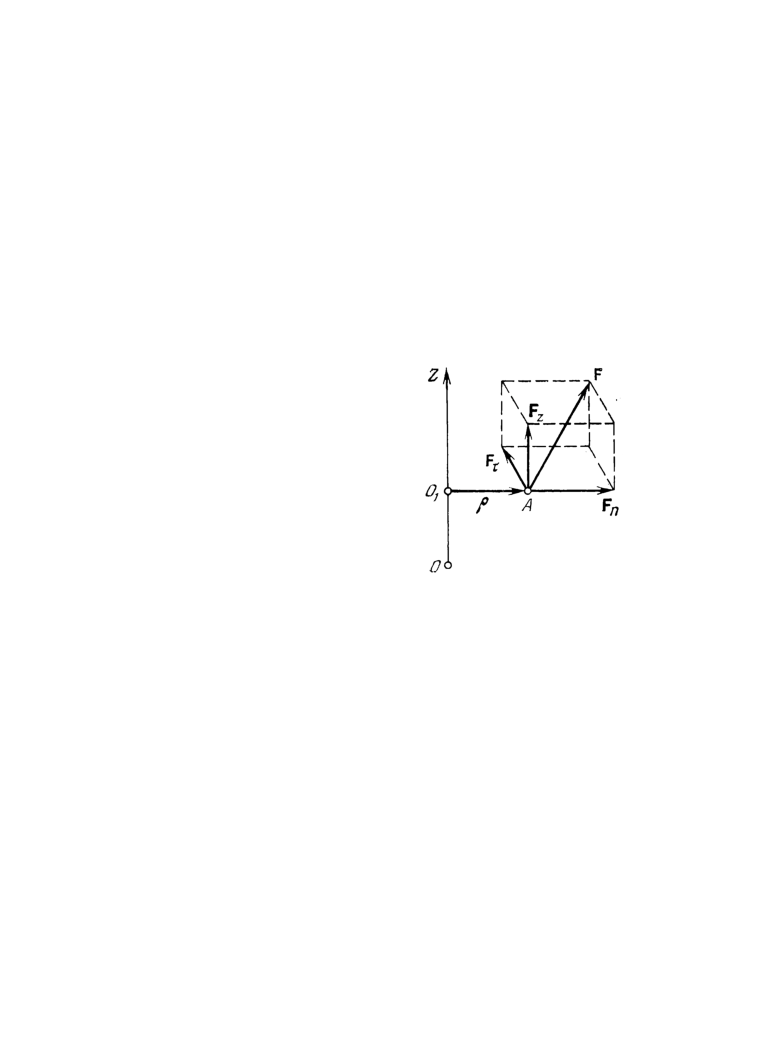
\includegraphics[width=0.8\textwidth,angle=-1]{figs/ch-04/fig-04-02.pdf}
%\input{figs/ch-03/fig-03-01}
%  \vspace{-13pt}
\caption{Resolving the components of the moment of force $\vb{M}$.\zhcap{力矩 $\vb{M}$ 的分量分解示意图。}
\label{fig-04-02}}
\end{marginfigure}

The moment of force $\vb{F}$ about axis $OZ$ is
\zhpar{力 $\vb{F}$ 对轴 $OZ$ 的力矩如下式所示。}
\begin{equation*}%
M_{z} = \qty[\pmb{\rho}\vb{F}_{\tau}]_{z}\,\, \textrm{and}\,\, \vb{M}_{z}=\qty[\pmb{\rho}\vb{F}_{\tau}].
\end{equation*}
Since vectors $\pmb{\rho}$ and $\vb{F}_{\tau}$ are perpendicular to each other
\zhpar{由于矢量 $\pmb{\rho}$ 与 $\vb{F}_{\tau}$ 相互垂直，故其模之间有如下关系。}
\begin{equation*}%
\abs{\vb{M}_{z}}= \abs{M_{z}} = \rho \abs{\vb{F}_{\tau}}.
\end{equation*}
The \redem{principal}, or \redem{resultant, moment} of a system of forces \redem{about a fixed axis $a$} is equal to the algebraic sum of the moments of all the forces of the system about this axis.
\zhpar{力系\redem{对定轴 $a$} 的\redem{主力矩}，或称\redem{合力矩}，等于该力系中全部力对该轴的力矩的代数和。}

\subsection{}\label{4.1.4} The \redem{angular momentum}, or \redem{moment of momentum, of a particle about fixed point $O$} (\redem{pole}) is the vector $\vb{L}$. It is equal to the vector product of radius vector $\vb{r}$, from point $O$ to the location of the particle, by vector $\vb{p}$ of its momentum:
\zhpar{质点对定点 $O$（\redem{极点}）的\redem{角动量}，又称\redem{动量矩}，是一个矢量 $\vb{L}$。它等于由点 $O$ 指向质点所在位置的位矢 $\vb{r}$ 与质点动量矢量 $\vb{p}$ 的矢积，如下式所示。}
\begin{equation*}%
\vb{L} = \qty[\vb{r\,p}] = \qty[\vb{r}m\vb{v}],
\end{equation*}
where $m$ and $\vb{v}$ are the mass and velocity of the particle.
\zhpar{式中 $m$ 和 $\vb{v}$ 分别为质点的质量和速度。}

The \redem{angular momentum of a system about fixed point $O$} is denoted by vector $\vb{L}$ and equals the vector sum of the angular momenta of all the particles of the system about the same point $O$:
\zhpar{质点系对定点 $O$ 的\redem{角动量}记为矢量 $\vb{L}$，它等于系统中全部质点对同一点 $O$ 的角动量的矢量和，如下式所示。}
\begin{equation*}%
\vb{L} = \sum_{i=1}^{n}\qty[\vb{r}_{i}\,\vb{p}_{i}] = \sum_{i=1}^{n}\qty[\vb{r}_{i}m_{i}\vb{v}_{i}],
\end{equation*}
where $m_{i}$, $\vb{r}_{i}$ and $\vb{v}_{i}$ are the mass, radius vector and velocity of the $i$-th particle, and $n$ is the total number of particles.
\zhpar{式中 $m_{i}$、$\vb{r}_{i}$ 和 $\vb{v}_{i}$ 分别为第 $i$ 个质点的质量、位矢和速度，$n$ 为质点总数。}

The \redem{angular momentum of a system about fixed axis $a$} is the scalar quantity $L_{a}$, equal to the projection on axis $a$ of vector $\vb{L}$, the angular momentum of the system about some point $O$ lying on this axis:
\zhpar{质点系对定轴 $a$ 的\redem{角动量}是一个标量 $L_{a}$，它等于质点系对该轴上某一点 $O$ 的角动量矢量 $\vb{L}$ 在轴 $a$ 上的投影，如下式所示。}
\begin{equation*}%
L_{a} = \sum_{i=1}^{n} \qty[\vb{r}_{i}m_{i}\vb{v}_{i}]_{a}.
\end{equation*}
The numerical value $L_{a}$ of the angular momentum is indepen­dent of the choice of the position of point $O$ along axis $a$.
\zhpar{角动量的数值 $L_{a}$ 与点 $O$ 在轴 $a$ 上位置的选取无关。}

\textbf{Note.} Sometimes the angular momentum of a system about a fixed axis $a$ is understood to mean the vector quantity $\vb{L}_{a}  = L_{a}\vb{i}_{a}$ where $\vb{i}_{a}$ is the unit vector of axis $a$.
\zhpar{注：有时质点系对定轴 $a$ 的角动量被理解为矢量 $\vb{L}_{a}  = L_{a}\vb{i}_{a}$，其中 $\vb{i}_{a}$ 为轴 $a$ 的单位矢量。}

\subsection{}\label{4.1.5} The \redem{angular momentum of a body rotating about a fixed point O} at the angular velocity is equal to:
\zhpar{绕固定点 $O$ 转动的刚体，以角速度转动时，其\redem{角动量}等于：}
\begin{equation*}%
\vb{L} = \int_{(m)} \qty[\vb{r}\vb{v}] \dd m = \int_{(m)} \qty[\vb{r}[\pmb{\omega}\vb{r}]] \dd m.
\end{equation*}
where $\vb{r}$ is the radius vector from point $O$ to an infinitely small (dement of the body of mass $\dd m$, and $\vb{v} = \qty[\pmb{\omega}\vb{r}]$ is the velocity of the element of the body. Since $\qty[\vb{r} \qty[\pmb{\omega}\vb{r}]] = r^{2}\pmb{\omega} - (\pmb{\omega}\vb{r}) \vb{r}$, vectors $\vb{L}$ and $\pmb{\omega}$ do not coincide in direction in the general case:
\zhpar{式中 $\vb{r}$ 为由定点 $O$ 指向刚体中质量为 $\dd m$ 的无限小微元的位矢，$\vb{v} = \qty[\pmb{\omega}\vb{r}]$ 为该微元的速度。由于 $\qty[\vb{r} \qty[\pmb{\omega}\vb{r}]] = r^{2}\pmb{\omega} - (\pmb{\omega}\vb{r}) \vb{r}$，一般情况下矢量 $\vb{L}$ 与 $\pmb{\omega}$ 的方向并不一致，其关系如下式所示。}
\begin{equation*}%
\vb{L} = \pmb{\omega} \int_{(m)} r^{2} \dd m - \int_{(m)} (\pmb{\omega}\vb{r}) \vb{r} \dd m.
\end{equation*}
The angular momentum of a body hinged at point $O$ and its angular velocity coincide in direction if the body rotates about one of its principal axes of inertia \ssect{4.2.4} passing through point $O$
\zhpar{绕铰接于点 $O$ 的刚体，若其绕通过点 $O$ 的惯性主轴之一（见\ssect{4.2.4}）转动，则其角动量与角速度方向一致，如下式所示。}
\begin{equation*}%
\vb{L} = \vb{I} \pmb{\omega},
\end{equation*}
where $\vb{I}$ is the moment of inertia \ssect{4.2.1} of the body about this principal axis.
\zhpar{式中 $\vb{I}$ 为刚体绕该惯性主轴的转动惯量（见\ssect{4.2.1}）。}
\subsection{}\label{4.1.6} The resultant moments $\vb{M}$ and $\vb{M}^{*}$ of a system of forces about two different fixed points $O$ and $O^{*}$ are related by the equation
\zhpar{力系对两个不同定点 $O$ 与 $O^{*}$ 的合力矩 $\vb{M}$ 与 $\vb{M}^{*}$ 之间的关系由下式给出。}
\begin{equation*}%
\vb{M} = \vb{M}^{*} + \qty[\vb{r}^{*}\vb{F}],
\end{equation*}
where $\vb{r}^{*}$ is the radius vector from origin $O$ to point $O^{*}$, and $\vb{F}$ is the principal vector of the system of forces being considered. If $\vb{F} = 0$ the resultant moment of the system of forces is the same about any fixed point: $\vb{M}^{*} = \vb{M}$. This, precisely, is the property possessed by a \redem{force couple}, or simply \redem{couple}, i.e. a system of two forces, equal in magnitude and directed along two parallel straight lines in opposite directions. The shortest (perpendicular) distance d between the lines of action of the forces is called the \redem{arm of the couple}. The moment, or torque, of a force couple is directed perpendicular to the plane of the forces, and its magnitude is equal to $M = Fd$, where $F$ is the magnitude of each of the forces of the couple.
\zhpar{式中 $\vb{r}^{*}$ 为由原点 $O$ 指向点 $O^{*}$ 的位矢，$\vb{F}$ 为所讨论力系的主矢。若 $\vb{F} = 0$，则力系对任一定点的合力矩均相同，即 $\vb{M}^{*} = \vb{M}$。正是\redem{力偶}（或简称\redem{偶}）具有这一性质。力偶是由大小相等、方向相反、作用线沿两条平行直线的两个力所组成的力系。两力作用线之间的最短（垂直）距离 $d$ 称为\redem{力偶臂}。力偶的力矩（或称转矩）垂直于力所在的平面，其大小为 $M = Fd$，式中 $F$ 为力偶中每个力的大小。}

The resultant moment $\vb{M}_{C}$ of all the forces acting on a mechan­ical system about the centre of mass \ssect{2.3.3} of this system is related to the resultant moment $\vb{M}$ of the same system of forces about fixed point $O$ by the equation
\zhpar{作用于力学系统的全部力对该系统质心 \ssect{2.3.3} 的合力矩 $\vb{M}_{C}$，与该力系对定点 $O$ 的合力矩 $\vb{M}$ 之间的关系由下式给出。}
\begin{equation*}%
\vb{M} = \vb{M}_{C} + \qty[\vb{r}_{C}\vb{F}],
\end{equation*}
where $\vb{r}_{C}$ is a radius vector from origin $O$ to point $C$, and $\vb{F}$ is the principal vector of the system of forces.
\zhpar{式中 $\vb{r}_{C}$ 为由原点 $O$ 指向点 $C$ 的位矢，$\vb{F}$ 为该力系的主矢。}

\subsection{}\label{4.1.7} The value of the angular momentum of a mechanical system about its centre of mass $C$ is the same for the absolute motion of the particles at the velocities (i.e. with respect to a fixed inertial frame of reference) and for the relative motion at the velocities $\vb{v}_{i}' = \vb{v}_{i} - \vb{v}_{C}$ (i.e. with respect to a frame of reference in translational motion with the origin of coordinates at point $C$):
\zhpar{质点系对其质心 $C$ 的角动量，无论是质点的绝对运动（速度为 $\vb{v}_{i}$，相对于固定惯性参考系），还是相对运动（速度为 $\vb{v}_{i}' = \vb{v}_{i} - \vb{v}_{C}$，相对于原点位于 $C$ 点、作平动的参考系），其值均相同，如下式所示。}
\begin{equation*}%
\sum_{i=1}^{n} \qty[\vb{r}_{i}m_{i} \vb{v}_{i}] = \sum_{i=1}^{n} \qty[\vb{r}_{i}'m_{i} \vb{v}_{i}'] = \vb{L}_{C},
\end{equation*}
where $\vb{r}_{i}' = - \vb{r}_{C}$ is the radius vector of the $i$-th particle in a frame of reference travelling together with the centre of mass.
\zhpar{式中 $\vb{r}_{i}' = - \vb{r}_{C}$ 为第 $i$ 个质点在随质心一同平动的参考系中的位矢。}

The relation between the values of the angular momentum $\vb{L}$ of a mechanical system about fixed point $O$ and $\vb{L}_{C}$ about the system's centre of mass is of the form
\zhpar{质点系对定点 $O$ 的角动量 $\vb{L}$ 与对质心的角动量 $\vb{L}_{C}$ 之间的关系具有如下形式。}
\begin{equation*}%
\vb{L} = \vb{L}_{C} + \qty[\vb{r}_{C}\vb{p}],
\end{equation*}
where $\vb{p} = \sum_{i=1}^{n} m_{i}\vb{v}_{i}$ is the momentum of the system in its 
absolute motion.
\zhpar{式中 $\vb{p} = \sum_{i=1}^{n} m_{i}\vb{v}_{i}$ 为质点系在绝对运动中的动量。}


\section{Moment of Inertia}
\label{sec-4.2}
\zhtitle{转动惯量}

\subsection{}\label{4.2.1} The \redem{moment of inertia of a mechanical system} about fixed axis $a$ is the physical quantity denoted by $I_{a}$ and equal to the sum of the products of the masses of all $n$ particles of the system by the squares of their normal distances from the axis:
\zhpar{质点系对定轴 $a$ 的\redem{转动惯量}是一个物理量，记作 $I_{a}$，它等于系统中全部 $n$ 个质点的质量与其到该轴法向距离平方的乘积之和，其表达式如下。}
\begin{equation*}%
I_{a} =  \sum_{i=1}^{n} m_{i} \rho_{i}^{2},
\end{equation*}
where $m_{i}$ and $\rho_{i}$ are the mass of the $i$-th particle and its normal distance from the axis.
\zhpar{式中 $m_{i}$ 和 $\rho_{i}$ 分别为第 $i$ 个质点的质量及其到该轴的法向距离。}

The moment of inertia of a body about fixed axis $a$ is
\zhpar{物体对定轴 $a$ 的转动惯量如下式所示。}
\begin{equation*}%
I_{a} =  \int_{(m)} \rho^{2} \dd m = \int_{(V)} \rho^{2} D \dd V,
\end{equation*}
where $\dd m = D \dd V$ is the mass of an infinitely small element of volume $\dd V$ of the body, $D$ is the density and $\rho$ is the normal distance from the element $\dd V$ to axis $a$.
\zhpar{式中 $\dd m = D \dd V$ 为物体中无限小体积元 $\dd V$ 的质量，$D$ 为密度，$\rho$ 为体积元 $\dd V$ 到轴 $a$ 的法向距离。}

If the body is homogeneous, i.e. its density is the same through­ out, then
\zhpar{若物体是均匀的，即密度处处相同，则有下式。}
\begin{equation*}%
I_{a} =  D \int_{(V)} \rho^{2} \dd V.
\end{equation*}
The moment of inertia $I_{a}$ is a measure of inertness of a body in its rotary motion about fixed axis $a$ \ssect{4.3.4}, in the same way that its mass is a measure of inertness of the body in its transla­tional motion.
\zhpar{转动惯量 $I_{a}$ 是物体绕定轴 $a$ 转动时惯性大小的量度（见\ssect{4.3.4}），正如质量是物体平动时惯性大小的量度一样。}

\subsection{}\label{4.2.2} The moment of inertia of a given body about some axis depends, not only on the mass, shape and size of the body, but also on the position of the body with respect to this axis. Ac­ cording to \redem{Steiner's theorem of parallel axes}, the moment of inertia $I$ of a body about an arbitrary axis is equal to the sum of its moment of inertia $I_{C}$ about a parallel axis through the centre of mass (or of inertia) of the body plus the product of the mass $m$ of the body by the square of the normal distance d between the two axes:
\zhpar{同一物体对某轴的转动惯量不仅取决于物体的质量、形状和大小，还取决于物体相对于该轴的位置。根据\redem{平行轴定理（施泰纳定理）}，物体对任一轴的转动惯量 $I$ 等于它对与该轴平行且通过物体质心（或惯量中心）的轴的转动惯量 $I_{C}$，加上物体质量 $m$ 与两轴之间法向距离 $d$ 的平方之积：}
\begin{equation*}%
I = I_{C} + md^{2}.
\end{equation*}

\clearpage
\subsection{}\label{4.2.3} The moments of inertia of certain homogeneous regularly shaped bodies about certain axes are listed in \tabl{4.1-mi-of-body}.
\zhpar{若干均匀且形状规则的物体对某些轴的转动惯量列于\tabl{4.1-mi-of-body}中。}

\begin{table*}[ht]
\caption{The moments of inertia of certain homogeneous regularly shaped bodies about certain axes.\zhcap{若干均匀规则形状物体对某些轴的转动惯量。}
\label{4.1-mi-of-body}}
\begin{small}
\begin{tabular}{p{3.75cm}p{3.75cm}p{1.5cm}}
\toprule
\hlblue{Body} & \hlblue{Position of axis $a$} & \hlblue{Moment of inertia $I_{a}$}\\
\midrule
Hollow thin-walled cir­cular cylinder of radius $R$ and mass $m$& Axis of the cylinder & $mR^{2}$ \\
Solid circular cylinder (or disk) of radius $R$ and mass $m$& Axis of the cylinder
& $mR^{2}/2$ \\
Solid sphere of radius $R$ and mass $m$ & Axis through the centre of the sphere & $2mR^{2}/5$ \\
Hollow thin-walled sphere of radius $R$ and mass $m$ & Axis through the centre of the sphere& $2mR^{2}/3$\\
Thin straight rod of length $l$ and mass $m$ & Axis perpendicular to the rod and through its centre along its length& $ml^{2}/12$\\
The same rod & Axis perpendicular to the rod and through one end of it& $ml^{2}/3$ \\
\bottomrule
\end{tabular}
\end{small}
\end{table*}
\clearpage

\subsection{}\label{4.2.4} The \redem{products of inertia of a body} about the axes of a rec­tangular Cartesian coordinate system are the quantities:
\zhpar{物体对直角笛卡儿坐标系各轴的\redem{惯量积}为下列各量：}
\begin{align*}%
I_{xy} & =  \int_{(m)} xy \dd m = \int_{(V)} xy\, D \dd V, \\
I_{xz} & =  \int_{(m)} xz \dd m = \int_{(V)} xz\, D \dd V, \\
I_{yz} & =  \int_{(m)} yz \dd m = \int_{(V)} yz\, D \dd V.
\end{align*}
where $x$, $y$ and $z$ are the coordinates of an infinitely small element of the body of volume $\dd V$, density $D$ and mass $m$.
\zhpar{式中 $x$、$y$ 和 $z$ 为物体中一个无限小单元的坐标，该单元的体积为 $\dd V$，密度为 $D$，质量为 $m$。}

Axis $OX$ is called the \redem{principal axis of inertia of the body} if the products of inertia $I_{xy}$ and $I_{xz}$ are simultaneously equal to zero. Three principal axes of inertia can be passed through each point of the body. The axes are mutually perpendicular.
\zhpar{若惯量积 $I_{xy}$ 与 $I_{xz}$ 同时等于零，则称 $OX$ 轴为物体的\redem{惯性主轴}。过物体中每一点都可以作出三条惯性主轴，它们彼此相互垂直。}

The moments of inertia of a body about the three principal axes of inertia, passed through an arbitrary point $O$ of the body, are called the \redem{principal moments of inertia of the body}.
\zhpar{物体对过其任一点 $O$ 的三条惯性主轴的转动惯量，称为物体的\redem{主转动惯量}。}

The principal axes of inertia, passing through the centre of mass of the body, are called the \redem{principal central axes of inertia of the body}, and the moments of inertia about these axes are called the \redem{principal central moments of inertia of the body}. An axis of symmetry of a homogeneous body is always one of its principal central axes of inertia.
\zhpar{通过物体质心的惯性主轴称为物体的\redem{主中心惯性轴}，对这些轴的转动惯量称为物体的\redem{主中心转动惯量}。均匀物体的对称轴总是其主中心惯性轴之一。}

\section{The Fundamental Law in the Dynamics of Rotary Motion}
\label{sec-4.3}
\zhtitle{转动动力学基本定律}

\subsection{}\label{4.3.1} It follows from Newton's laws that the first derivative with respect to time $t$ of the angular momentum $\vb{L}$ of a mechan­ical system about any fixed point 0 is equal to the resultant moment $M^{\textrm{ext}}$ of all the external forces, applied to the system, about the same point $O$:
\zhpar{由牛顿定律可知，质点系对任一定点 $O$ 的角动量 $\vb{L}$ 对时间 $t$ 的一阶导数，等于该系统所受全部外力对同一点 $O$ 的合力矩 $M^{\textrm{ext}}$：}
\begin{equation*}%
\dv{\vb{L}}{t} = M^{\textrm{ext}}.
\end{equation*}
This equation expresses the \redem{law of the variation of angular mo­mentum of the system}. It is valid, in particular, for a rigid body, hinged at point $O$ and rotating about it. In this case, the equation expresses the \redem{fundamental law of dynamics of a rigid body rotating about a fixed point}.
\zhpar{该方程表示\redem{质点系角动量的变化定律}。它尤其适用于绕铰接于点 $O$ 的刚体。在这种情况下，该方程即为\redem{绕定点转动的刚体动力学基本定律}。}

In terms of the projections on the axes of a fixed rectangular Cartesian coordinate system with its origin at point $O$, the law for the variation of the angular momentum is written in the form:
\zhpar{若取原点位于 $O$ 点的固定笛卡儿直角坐标系，则角动量变化定律在各坐标轴上的投影形式为：}
\begin{equation*}%
\dv{L_{x}}{t} = M^{\textrm{ext}}_{x}, \,\,\dv{L_{y}}{t} = M^{\textrm{ext}}_{y}, \,\,\dv{L_{z}}{t} = M^{\textrm{ext}}_{z}.
\end{equation*}

Here $L_{x}, \,L_{y}, \,L_{z}, \,M^{\textrm{ext}_{x}}, \,M^{\textrm{ext}}_{x}, \,M^{\textrm{ext}}_{y}\,M^{\textrm{ext}}_{z}$ are the angular mo­menta of the system and the resultant moments of the external forces about the corresponding coordinate axes.
\zhpar{式中 $L_{x}, \,L_{y}, \,L_{z}, \,M^{\textrm{ext}_{x}}, \,M^{\textrm{ext}}_{x}, \,M^{\textrm{ext}}_{y}\,M^{\textrm{ext}}_{z}$ 分别为质点系的角动量以及外力对相应坐标轴的合力矩。}



\subsection{}\label{4.3.2} \hlblue{Example.} The \redem{regular precession of a gyroscope} due to its gravitational force. A \redem{gyroscope (symmetrical gyroscope)} is a rigid body spinning (rotating rapidly) about its axis of symmetry that can change its position in space. A gyroscope has three degrees of freedom \ssect{1.5.6} if it is mounted at fixed point $O$, which lies on its axis and is called the \redem{centre of suspension of the gyroscope}. 
\zhpar{\hlblue{例题。}重力引起的陀螺仪的\redem{规则进动}。\redem{陀螺仪}（或称\redem{对称陀螺仪}）是绕其对称轴高速自转、且其在空间中的位置可以改变的刚体。若将陀螺仪安装在其轴线上的定点 $O$ 处，则它具有三个自由度（见\ssect{1.5.6}），该定点称为\redem{陀螺仪的悬挂中心}。}
\begin{marginfigure}%[!ht]
%\begin{wrapfigure}{r}{0.5\linewidth}
\centering
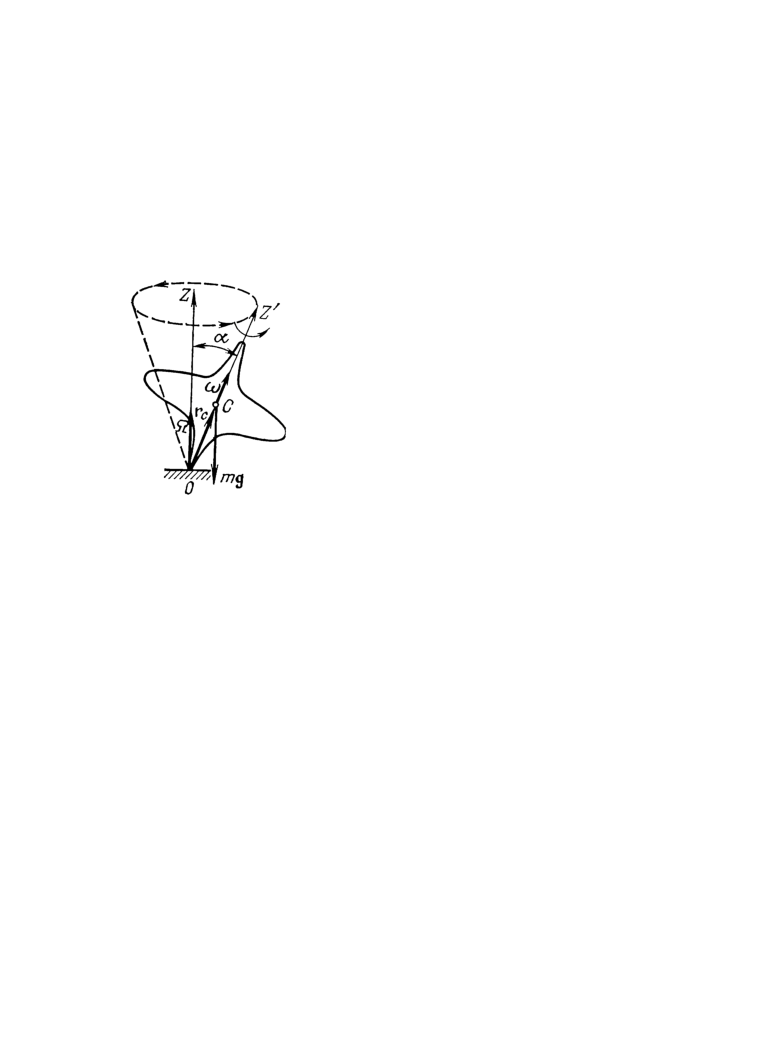
\includegraphics[width=0.6\textwidth,angle=-1]{figs/ch-04/fig-04-03.pdf}
%\input{figs/ch-03/fig-03-01}
%  \vspace{-13pt}
\caption{Analysing the rotary motion of a heavy gyroscope or a top.\zhcap{分析重陀螺仪或陀螺的转动运动。}
\label{fig-04-03}}
\end{marginfigure}

If the centre of suspension coincides with the centre of gravity $C$ \ssect{7.3.2} of the gyroscope, the gyroscope is said to be \redem{balanced}: the force of gravity does not affect its state of rotation. Otherwise, it is said to be a \redem{heavy gyroscope}, or top (\figr{fig-04-03}). Owing to the action of the moment of gravitational force about point $O$
\zhpar{若悬挂中心与陀螺仪的重心 \ssect{7.3.2} $C$ 重合，则称该陀螺仪为\redem{平衡陀螺仪}：重力不影响其转动状态。否则，称之为\redem{重陀螺仪}，或称陀螺（见\figr{fig-04-03}）。由于重力对点 $O$ 的力矩作用，有下式成立。}
\begin{equation*}%
M^{\textrm{ext}} = \qty[\vb{r}_{C}m \vb{g}],
\end{equation*}
a heavy gyroscope rotates about this point so that its axis $OZ'$ rotates uni­formly about vertical axis $OZ$ describ­ing a conical surface (shown by dashed lines in \figr{fig-04-03}). Such motion of the gyroscope is called \redem{regular precession}. If the angular velocity of precession $\Omega \ll \omega$ (where $\omega$ is the spin angular velocity or, simply, spin velocity of the gyroscope about its axis of symmetry $OZ'$), it can be assumed with some approximation that the angular momentum $\vb{L}$ of the gyroscope about point $O$ is directed along axis $OZ'$ of the gyroscope and equals
\zhpar{重陀螺仪绕该点转动，使其轴 $OZ'$ 绕竖直轴 $OZ$ 匀速转动，并描出一个圆锥面（\figr{fig-04-03} 中虚线所示）。陀螺仪的这种运动称为\redem{规则进动}。若进动角速度 $\Omega \ll \omega$（其中 $\omega$ 为陀螺仪绕其对称轴 $OZ'$ 的自转角速度，或简称自转速度），则可以近似地认为陀螺仪对点 $O$ 的角动量 $\vb{L}$ 沿陀螺仪的轴 $OZ'$ 方向，并等于下式所示的值。}
\begin{equation*}%
\vb{L} = I \pmb{\omega},
\end{equation*}
where $I$ is the moment of inertia of the gyroscope about axis $OZ'$. Hence
\zhpar{式中 $I$ 为陀螺仪绕轴 $OZ'$ 的转动惯量。由此得}
\begin{equation*}%
\dv{\vb{L}}{t} = \qty[\vb{r}_{C}m\vb{g}] = \qty[\frac{\vb{r}_{C}}{I \omega_{z'}} \vb{L} m\vb{g}] = \qty[\pmb{\Omega}\vb{L}],
\end{equation*}
where $\pmb{\Omega} = - m\vb{r}_{C}g/I\omega_{z'}$, is the angular velocity of precession, and $\omega_{z'} = \omega$ in the case shown in \figr{fig-04-03}. The greater the spin angular velocity of the gyroscope the slower its precession. 
\zhpar{式中 $\pmb{\Omega} = - m\vb{r}_{C}g/I\omega_{z'}$ 为进动角速度，且在 \figr{fig-04-03} 所示的情形中 $\omega_{z'} = \omega$。陀螺仪的自转角速度越大，其进动就越慢。}

\subsection{}\label{4.3.3} The kinetic energy of a rigid body rotating about a fixed point at the angular velocity $\pmb{\omega}$ is 
\zhpar{绕定点以角速度 $\pmb{\omega}$ 转动的刚体，其动能为：}
\begin{equation*}%
E_{k} = \frac{I \pmb{\omega}^{2}}{2},
\end{equation*}
where $I$ is the moment of inertia of the body about the instan­taneous axis of rotation \ssect{1.5.6}.
\zhpar{式中 $I$ 为刚体绕瞬时转轴（见\ssect{1.5.6}）的转动惯量。}

An element of work done in the infinitely short time interval $\dd t$ by force $\vb{F}$ acting on the body is
\zhpar{在无限短的时间间隔 $\dd t$ 内，作用于刚体上的力 $\vb{F}$ 所做的元功为：}
\begin{equation*}%
\delta W = \vb{M} \pmb{\omega} \dd t = \vb{M} \dd \pmb{\varphi}  = M_{\omega} \dd \varphi,
\end{equation*}
where $\vb{M} = [\vb{rF}]$ is the moment of force $\vb{F}$ about point $O$ ($\vb{r}$ is the radius vector from point $O$ to the point of application of force $\vb{F}$), $\dd \varphi  = \omega \dd t$ and $\dd \pmb{\varphi} = \pmb{\omega} \dd t$ are the angle of rotation and the vector of an element of rotation of the body in the time interval $\dd t$, and $M_{\omega}$ is the moment of force $\vb{F}$ about an instantaneous axis of rotation ($\vb{M}_{\omega}$ equal to the projection of vector $\vb{M}$ on the direction of vector $\omega$).
\zhpar{式中 $\vb{M} = [\vb{rF}]$ 为力 $\vb{F}$ 对定点 $O$ 的力矩（$\vb{r}$ 为由点 $O$ 指向力 $\vb{F}$ 作用点的位矢），$\dd \varphi = \omega \dd t$ 与 $\dd \pmb{\varphi} = \pmb{\omega} \dd t$ 分别为时间间隔 $\dd t$ 内刚体的转角与转动元矢量，$M_{\omega}$ 为力 $\vb{F}$ 对瞬时转轴的力矩（$\vb{M}_{\omega}$ 等于矢量 $\vb{M}$ 在 $\pmb{\omega}$ 方向上的投影）。}

The change in the kinetic energy of a rotating rigid body during the time interval $\dd t$ is equal to the work done by the external forces:
\zhpar{在时间间隔 $\dd t$ 内，转动刚体动能的改变量等于外力所做的功：}
\begin{equation*}%
\dd E_{k} = M^{\textrm{ext}}_{\omega} \dd \varphi,
\end{equation*}
where is the resultant moment \ssect{4.1.3} of external forces about an instantaneous axis of rotation of the body.
\zhpar{式中所指为外力对刚体瞬时转轴的合力矩（见\ssect{4.1.3}）。}

\subsection{}\label{4.3.4} If a rigid body rotates about fixed axis $OZ$ at the angular velocity $\omega$, its angular momentum about this axis is
\zhpar{若刚体绕定轴 $OZ$ 以角速度 $\omega$ 转动，则其对该轴的角动量为：}
\begin{equation*}%
L_{z} = I_{z} \omega_{z}\,\, \textrm{and}\,\, \vb{L}_{z} = I_{z}\pmb{\omega}.
\end{equation*}
Here $I_{z}$ is the moment of inertia of the body about axis $OZ$ and does not change with time $(I_{z}\,= \,\textrm{const})$, and $\abs{\omega_{z}} = \omega > 0$ ($\omega_{z} = \omega$ if vector $\pmb{\omega}$ and the unit vector of axis $OZ$ coincide in direction, otherwise $\omega_{z} = - \omega$).
\zhpar{式中 $I_{z}$ 为刚体对轴 $OZ$ 的转动惯量，它不随时间改变（$I_{z}\,= \,\textrm{const}$），且 $\abs{\omega_{z}} = \omega > 0$（若矢量 $\pmb{\omega}$ 与轴 $OZ$ 的单位矢量方向一致，则 $\omega_{z} = \omega$，否则 $\omega_{z} = - \omega$）。}

The \redem{fundamental law in the dynamics of a rigid body rotating about fixed axis $OZ$ is}
\zhpar{刚体绕定轴 $OZ$ 转动时的\redem{动力学基本定律}为：}
\begin{equation*}%
I_{z} = \dv{\pmb{\omega}}{t} =  \vb{M}^{\textrm{ext}}_{z} \,\, \textrm{or} \,\, \pmb{\varepsilon} = \frac{1}{I_{z}} \vb{M}^{\textrm{ext}}_{z},
\end{equation*}
where $\pmb{\varepsilon} = \dv*{\pmb{\omega}}{t}$ is the angular acceleration of the body.
\zhpar{式中 $\pmb{\varepsilon} = \dv*{\pmb{\omega}}{t}$ 为刚体的角加速度。}

It is evident from the preceding equation that the moment of inertia of a rigid body about some fixed axis is a measure of inertness of the body in its rotation about the given axis: the greater the moment of inertia of the body, the less the angular acceleration it acquires under the action of the same moment of
external forces.
\zhpar{由上式可以看出，刚体对某定轴的转动惯量是刚体绕该轴转动时惯性大小的量度：转动惯量越大，在相同的外力矩作用下所获得的角加速度就越小。}

\subsection{}\label{4.3.5} The kinetic energy of a rigid body rotating about fixed axis $OZ$ at the angular velocity $\omega$ is
\zhpar{刚体绕定轴 $OZ$ 以角速度 $\omega$ 转动时，其动能为：}
\begin{equation*}%
E_{k} =  \frac{1}{2} I_{z} \omega^{2}.
\end{equation*}
An element of work done during the infinitely short time $\dd t$ by force $\vb{F}$ applied to the body is
\zhpar{在无限短的时间 $\dd t$ 内，作用于刚体上的力 $\vb{F}$ 所做的元功为：}
\begin{equation*}%
\delta W = \vb{M}_{z} \pmb{\omega} \dd t = M_{z} \dd \varphi,
\end{equation*}
where $M_{z}$ is the moment of force $\vb{F}$ about the axis $OZ$ of rota­tion (the unit vector of axis $OZ$ coincides in direction with vector $\pmb{\omega}$).
\zhpar{式中 $M_{z}$ 为力 $\vb{F}$ 对转轴 $OZ$ 的力矩（轴 $OZ$ 的单位矢量与矢量 $\pmb{\omega}$ 方向一致）。}

The change in the kinetic energy of a rigid body during the time interval $\dd t$ is equal to the work done by the external forces during this interval:
\zhpar{在时间间隔 $\dd t$ 内，转动刚体动能的改变量等于该时间间隔内外力所做的功：}
\begin{equation*}%
\dd E_{k} = M^{\textrm{ext}}_{z} \dd \varphi,
\end{equation*}
where $M^{\textrm{ext}}_{z}$ is the resultant moment of external forces about the axis of rotation of the body.
\zhpar{式中 $M^{\textrm{ext}}_{z}$ 为外力对刚体转轴的合力矩。}

\subsection{}\label{4.3.6} The motion of a free rigid body satisfies the following two differential equations:
\zhpar{自由刚体的运动满足下列两个微分方程：}
\begin{equation*}%
\dv{t}(m\vb{v}_{C}) = \vb{F}^{\textrm{ext}} \,\, \textrm{and}\,\,\dv{\vb{L}_{C}}{t} = \vb{M}^{\textrm{ext}}_{C}.
\end{equation*}
Here $m$ is the mass of the body, $\vb{v}_{C}$ is the velocity of its centre of mass $C$, $ \vb{F}^{\textrm{ext}}$ is the principal vector of external forces applied
to the body \ssect{2.5.2}, $\vb{M}^{\textrm{ext}}_{C}$ is the resultant moment of external forces about point $C$ \ssect{4.1.6}, and $\vb{L}_{C}$ is the angular momentum about the same point $C$ \ssect{4.1.7}.
\zhpar{式中 $m$ 为刚体的质量，$\vb{v}_{C}$ 为其质心 $C$ 的速度，$\vb{F}^{\textrm{ext}}$ 为作用于刚体上的外力的主矢（见\ssect{2.5.2}），$\vb{M}^{\textrm{ext}}_{C}$ 为外力对质心 $C$ 的合力矩（见\ssect{4.1.6}），$\vb{L}_{C}$ 为刚体对同一点 $C$ 的角动量（见\ssect{4.1.7}）。}

The first equation describes translational motion of the free body at the velocity of its centre of mass \ssect{2.5.3}. The second equation follows from the law of the variation of angular momentum \ssect{4.3.1} and describes the rotation of a rigid body about its centre of mass \ssect{1.5.9}.
\zhpar{第一个方程描述了自由刚体以其质心速度作平动的运动。第二个方程由角动量变化定律（见\ssect{4.3.1}）导出，描述刚体绕其质心的转动（见\ssect{1.5.9}）。}

\subsection{}\label{4.3.7} The kinetic energy of a free rigid body can be deter­ mined on the basis of Koenig's theorem \ssect{3.2.4}:
\zhpar{自由刚体的动能可以根据柯尼希定理（见\ssect{3.2.4}）求得：}
\begin{equation*}%
E_{k} = \frac{mv_{C}^{2}}{2} + \frac{I_{C}\omega^{2}}{2}.
\end{equation*}
where $I_{C}$ is the moment of inertia of the body about an instan­taneous axis of rotation passing through its centre of mass $C$, and $\omega$ is the angular velocity of the body. In the general case, the instantaneous axis is displaced in the body and the moment of inertia $I_{C}$ varies with time. The value of $I_{C}$ is constant if the body is in plane motion \ssect{1.5.9}.
\zhpar{式中 $I_{C}$ 为刚体对通过其质心 $C$ 的瞬时转轴的转动惯量，$\omega$ 为刚体的角速度。一般情况下，瞬时轴在刚体内发生位移，转动惯量 $I_{C}$ 随时间变化。若刚体做平面运动（见\ssect{1.5.9}），则 $I_{C}$ 的值保持不变。}

\hlblue{Example.} The kinetic energy of a homogeneous circular cylinder rolling down an inclined plane without slipping. The cylinder has plane motion because all of its points travel in vertical planes that are parallel to one another. The cylinder travels with translational motion at the velocity $\vb{v}_{C}$ directed along the inclined plane, and rotates about its axis ($I_{C} = mR^{2}/2$, where $m$ and $R$ are the mass and radius of the cylinder) at the angular velocity $\omega$. From the condition that the cylinder rolls without slipping it follows that the instantaneous veloci­ties of the points of contact between the cylinder and inclined plane equal zero, i.e. $\omega = v_{C}/R$. Hence, the kinetic energy of the rolling cylinder is
\zhpar{\hlblue{例题。}一个均匀圆柱体无滑动地沿斜面滚下时的动能。圆柱体做平面运动，因为其所有点都在彼此平行的竖直平面内运动。圆柱体以沿斜面方向的速度 $\vb{v}_{C}$ 作平动，并以角速度 $\omega$ 绕其轴线转动（$I_{C} = mR^{2}/2$，其中 $m$ 和 $R$ 分别为圆柱体的质量和半径）。由圆柱体无滑动滚动的条件可知，其与斜面接触点的瞬时速度为零，即 $\omega = v_{C}/R$。因此，滚动圆柱体的动能为：}
\begin{equation*}%
E_{k} = \frac{mv_{C}^{2}}{2} + \frac{I_{C}\omega^{2}}{2} = \frac{3}{4}mv_{C}^{2}.
\end{equation*}


\section{Law of Conservation of Angular Momentum}
\label{sec-4.4}
\zhtitle{角动量守恒定律}

\subsection{}\label{4.4.1} The \redem{law of the conservation of angular momentum} can be formulated as follows: the angular momentum of a closed system \ssect{2.2.4} about any fixed point remains constant with time, i.e.
\zhpar{\redem{角动量守恒定律}可表述如下：封闭系统（见\ssect{2.2.4}）对任一定点的角动量不随时间改变，即}
\begin{equation*}%
\dv{\vb{L}}{t} \equiv 0 \,\, \textrm{and} \,\, \vb{L} = \textrm{const}.
\end{equation*}
Accordingly, the angular momentum of a closed system about its centre of mass \ssect{4.1.7} remains constant with time:
\zhpar{因此，封闭系统对其质心（见\ssect{4.1.7}）的角动量同样不随时间改变：}
\begin{equation*}%
\dv{\vb{L_{C}}}{t} \equiv 0 \,\, \textrm{and} \,\, \vb{L_{C}} = \textrm{const}.
\end{equation*}
Like the laws of conservation of momentum and energy, the law of conservation of angular momentum is of significance far beyond the scope of classical mechanics. It belongs to the most Fundamental of physical laws because it is associated with a definite symmetry property of space: its isotropy. The \redem{isotropy of space} is manifested in the fact that the physical properties and laws of motion of a closed system are independent of the direction chosen for the coordinate axes in an inertial frame of reference. This means that these properties and laws do not change when the closed system is turned as a whole through any angle in space.
\zhpar{与动量守恒定律和能量守恒定律一样，角动量守恒定律的意义远远超出经典力学的范围。它是最基本的物理定律之一，因为它与空间的一种特定对称性——\redem{空间的各向同性}——相联系。空间的各向同性表现为：在惯性参考系中，封闭系统的物理性质和运动规律与坐标轴的方向选取无关。这意味着，当封闭系统作为一个整体在空间中转过任意角度时，这些性质和规律都不会改变。}

According to modern concepts, not only particles and bodies can have an angular momentum, hut fields as well. Elementary particles and systems built from them (for instance, atomic nuclei) can have an angular momentum that is not related to their motion in space and is called their spin (\tabl{tab-43.1}). 
\zhpar{根据现代概念，不仅质点和物体可以具有角动量，场也同样可以具有角动量。基本粒子以及由其组成的系统（例如原子核）也可以具有角动量，这种角动量与它们在空间中的运动无关，称为其\redem{自旋}（见\tabl{tab-43.1}）。}

\subsection{}\label{4.4.2} With respect to systems that can be described by classical (Newtonian) mechanics, the law of conservation of angular momentum can be regarded as a consequence of Newton's laws. For a closed mechanical system, the resultant moment of exter­nal forces about any fixed point (as well as about the centre of mass of the system) is identically zero: $\vb{M}^{\textrm{ext}} \equiv 0$ (consequently, $\vb{M}^{\textrm{ext}}_{C} \equiv 0$, see \ssect{4.1.6}, where $\vb{F} = \vb{F}^{\textrm{ext}} \equiv 0$) and the law of conservation of angular momentum follows from \ssect{4.3.1}:
\zhpar{对于可以用经典（牛顿）力学描述的系统，角动量守恒定律可以看作牛顿定律的推论。对于封闭的力学系统，外力对任一定点（以及对系统质心）的合力矩恒等于零：$\vb{M}^{\textrm{ext}} \equiv 0$（因此 $\vb{M}^{\textrm{ext}}_{C} \equiv 0$，参见\ssect{4.1.6}，此时 $\vb{F} = \vb{F}^{\textrm{ext}} \equiv 0$），由\ssect{4.3.1}即可得出角动量守恒定律：}
\begin{equation*}%
\vb{L} = \sum_{i=1}^{n} \qty[\vb{r}_{i} m_{i} \vb{v}_{i}] = \textrm{const}.
\end{equation*}
where $m_{i},\vb{r}_{i}$ and $\vb{v}_{i}$ are the mass, radius vector and velocity of the $i$-th particle of the system, which consists of $n$ such particles. 
\zhpar{式中 $m_{i}$、$\vb{r}_{i}$ 和 $\vb{v}_{i}$ 分别为由 $n$ 个这样的质点组成的系统中第 $i$ 个质点的质量、位矢和速度。}

Accordingly (see \ssect{4.1.7} and \ssect{2.5.3}),
\zhpar{相应地（参见\ssect{4.1.7}和\ssect{2.5.3}），有如下关系：}
\begin{equation*}%
\vb{L}_{C} = \sum_{i=1}^{n} \qty[\vb{r}_{i}' m_{i} \vb{v}_{i}'] = \sum_{i=1}^{n} \qty[\vb{r}_{i} m_{i} \vb{v}_{i}] =\textrm{const}.
\end{equation*}
where $\vb{r}_{i}' = \vb{r}_{i} - \vb{r}_{C}$, and $\vb{v}_{i}' = \vb{v}_{i} - \vb{v}_{C}$ and $\vb{r}_{C},\,\vb{v}_{C}$ are the radius vector and velocity of the system's centre of mass.
\zhpar{式中 $\vb{r}_{i}' = \vb{r}_{i} - \vb{r}_{C}$，$\vb{v}_{i}' = \vb{v}_{i} - \vb{v}_{C}$，$\vb{r}_{C}$、$\vb{v}_{C}$ 分别为质点系质心的位矢和速度。}

\subsection{}\label{4.4.3} If a system is not closed, but the external forces acting on it are such that their resultant moment about fixed point $O$ is identically zero $ (\vb{M}^{\textrm{ext}} \equiv 0)$, then, according to Newton's laws \ssect{4.3.1}, the angular momentum of the system about the same point $O$ remains constant with time: $\vb{L} = \textrm{const}$. This condition is practically complied with, for example, by a bal­anced gyroscope \ssect{4.3.2} with three degrees of freedom, if the moment of the friction force in its suspension is sufficiently small.
\zhpar{若系统不封闭，但作用于其上的外力使其对定点 $O$ 的合力矩恒等于零（$\vb{M}^{\textrm{ext}} \equiv 0$），则根据牛顿定律（见\ssect{4.3.1}），系统对同一点 $O$ 的角动量保持不变：$\vb{L} = \textrm{const}$。例如，只要其悬挂处的摩擦力矩足够小，具有三个自由度（见\ssect{4.3.2}）的平衡陀螺仪实际上就能满足这一条件。}

If the stand of the gyroscope, holding its centre of suspension at rest, is turned in any way, the axis of the gyroscope retains its orientation with respect to a fixed inertial frame of reference.\sidenote[][-2cm]{It is assumed that vector $\vb{L}$ is directed along the axis of the gyroscope. Otherwise, a free gyroscope has a precessional motion: its axis describes a circular conical surface whose vertex is at the centre of suspension and whose axis is directed along the vector $\vb{L} = \textrm{const}$.}
\zhpar{若使陀螺仪的悬挂中心保持静止的支架以任意方式转动，则陀螺仪的轴相对于固定惯性参考系保持其方向不变。}
\zhpar{注：假定矢量 $\vb{L}$ 沿陀螺仪的轴线方向。否则，自由陀螺仪将作进动运动：其轴描出一个圆锥面，该圆锥面的顶点位于悬挂中心，其轴线沿矢量 $\vb{L} = \textrm{const}$ 的方向。}

Usually $\vb{M}^{\textrm{ext}} \nequiv 0$ and $\vb{L} \neq \textrm{const}$. But if the resultant moment of external forces about any fixed axis passing through point $O$ is identically zero, the angular momentum of the system about
this axis remains constant with time. For instance, if $M^{\textrm{ext}}_{z}\equiv 0$, then $L_{z} = \textrm{const}$.
\zhpar{通常情况下 $\vb{M}^{\textrm{ext}} \nequiv 0$，且 $\vb{L} \neq \textrm{const}$。但是，若外力对通过点 $O$ 的任一定轴的合力矩恒等于零，则系统对该轴的角动量保持不变。例如，若 $M^{\textrm{ext}}_{z}\equiv 0$，则 $L_{z} = \textrm{const}$。}

If the system rotates about fixed axis $OZ$ and the resultant moment of external forces about this axis $M^{\textrm{ext}}_{z} \equiv 0$, the angular momentum of the system about the axis of rotation remains constant with time:
\zhpar{若系统绕定轴 $OZ$ 转动，且外力对该轴的合力矩 $M^{\textrm{ext}}_{z} \equiv 0$，则系统对转轴的角动量保持不变，即：}
\begin{equation*}%
I_{z} \omega = \textrm{const.},
\end{equation*}
where $\omega$ and $I_{z}$ are the angular velocity and moment of inertia of the system.
\zhpar{式中 $\omega$ 与 $I_{z}$ 分别为系统的角速度与转动惯量。}

If the action of internal forces, as well as external forces that comply with the condition $M^{\textrm{ext}}_{z}\equiv 0$, leads to deformation of the system, changing its moment of inertia $I_{z}$, the angular velocity $\omega$ correspondingly increases or decreases.
\zhpar{若内力的作用，以及满足条件 $M^{\textrm{ext}}_{z}\equiv 0$ 的外力，使系统发生形变从而改变其转动惯量 $I_{z}$，则角速度 $\omega$ 相应地增大或减小。}

\subsection{}\label{4.4.4} \redem{Free axes of a body} are ones about which a free rigid body \ssect{2.2.3} can rotate at constant angular velocity $\pmb{\omega}$ in the absence of all external action. Such rotation of a body is said to be \redem{free}, or \redem{inertial rotation}. The free axes of a body coincide with its
principal central axes of inertia \ssect{4.2.4}. In the general case, the values $I_{1}$, $I_{2}$ and $I_{3}$ of the principal central moments of inertia \ssect{4.2.4} differ. The free rotation of such a body (for ex­ ample, a homogeneous rectangular parallelepiped with edges of different length) is accomplished practically only about two free axes, corresponding to the extreme values of the principal central moments of inertia -- the maximum and minimum val­ues. The rotation of the body about its third principal central axis, corresponding to the intermediate value of the moment of inertia of the body, proves to be unstable: even very small external action is capable of leading to substantial deviation of the instantaneous axis of rotation from its initial direction in the body.
\zhpar{\redem{物体的自由轴}是指在没有任何外部作用时，自由刚体能够以恒定角速度 $\pmb{\omega}$ 绕其转动的轴。这种转动称为\redem{自由转动}，或\redem{惯性转动}。物体的自由轴与其主中心惯性轴重合。一般情况下，三个主中心转动惯量 $I_{1}$、$I_{2}$、$I_{3}$ 各不相同。这类物体（例如边长各不相同的均匀长方体）实际上只能绕两个自由轴自由转动，它们分别对应主中心转动惯量的极大值和极小值。绕其第三个主中心轴（对应物体转动惯量的中间值）的转动是不稳定的：即使很小的外部作用，也能使瞬时转轴相对其在物体内的初始方向产生明显偏离。}

If the values of two principal central moments of inertia of a body are equal: $I_{1} = I_{2} \neq I_{3} $, stable free rotation of such a body (for instance, a homogeneous circular cylinder) is possi­ble only about the free axis corresponding to the third, differing value $I_{3}$ of the moment of inertia. For a homogeneous circular cylinder such a free axis is its axis of symmetry. But if a long thin cylinder is rotated by means of a string secured to one end, stable rotation of the cylinder can be accomplished about the free axis corresponding to the maximum value of its moment of inertia. This free axis is perpendicular to the axis of symmetry
of the cylinder.
\zhpar{若物体的两个主中心转动惯量相等，即 $I_{1} = I_{2} \neq I_{3}$，则这种物体（例如均匀圆柱体）只能绕与第三个不同值 $I_{3}$ 对应的自由轴作稳定的自由转动。对于均匀圆柱体，这一自由轴即为其对称轴。但是，若用一端系住的细绳转动一根细长圆柱体，则可以使其绕对应于其最大转动惯量的自由轴作稳定转动。该自由轴与圆柱体的对称轴垂直。}


%\begin{equation*}%
%\vb{F}= \sum_{i=1}^{n} \vb{F_{i}}
%\end{equation*}

%\end{wrapfigure}

%\begin{align*}%
%m\vb{a} = \vb{F}\,\,\textrm{and}\,\, \vb{F}_{ki} = - \vb{F}_{ik}\,\, \intertext{(in reference frame $K$)}\\
%m'\vb{a}' = \vb{F}'\,\,\textrm{and}\,\, \vb{F}_{ki}' = - \vb{F}_{ik}'\,\, \intertext{(in reference frame $K'$)}
%\end{align*}
